\documentclass[12pt,letterpaper,oneside]{memoir}

%%% Resets
% memoir defines footruleskip, we want fancyhdr's
\let\footruleskip\undefined
\DisemulatePackage{setspace}

%%% Packages
\usepackage{fancyhdr}
\usepackage{hyperref}
\usepackage{lastpage}
\usepackage{setspace}

%%% Headers/Footers
\pagestyle{fancyplain}
\fancyhf{}
\fancyheadoffset[r]{.01in}
\fancyhead[R]{Getting Lost / Scott-Clary / \thepage\ of \pageref{LastPage}}

%%% Font
\renewcommand*\rmdefault{ptm}
\renewcommand*\ttdefault{pcr}
\hypersetup{
    colorlinks,
    citecolor=black,
    filecolor=black,
    linkcolor=black,
    urlcolor=black
}

%%% Spacing
\onehalfspacing
\usepackage[top=1in, bottom=1in, right=1in, left=1in]{geometry}

%%% Commands
\newcommand\secdiv{
  \begin{center}
    \#
  \end{center}
}
\newcommand\ptCollin{aca973d7 }
\newcommand\ptRJ{0224ebe8 }

%%% Title
\title{Getting Lost}
\author{Madison Scott-Clary}

\begin{document}
  \maketitle

  \newpage

  \tableofcontents

  \part{}

  Many people, I suspect, use the idiom, ``Hindsight is twenty-twenty'' in a way that is better served by other, more appropriate words or phrases.   The sense in which I hear it most commonly used is perhaps more adequately covered by the beautiful portmanteau, ``regretrospect''.  That is, now that things are said and done, I respect a lot of what happened during this adventure.

Also, it's my second favorite portmanteau after ``congratudolences'' and really ought to see wider use.

No, I think ``hindsight is twenty-twenty'' is better reserved for cases when seemingly unrelated occurrences come together to form an outcome that seems to be greater than the sum of the parts.  It fits best when you look back at your life and disparate, unconnected events come together to make the situation you find yourself in now.

I came out to myself and my (at the time) fianc\'ee as transgender over a process of several months.  It began sometime in 2010 or so, when I started to feel like I was able to put words to the things that were making me feel bad.  I began by identifying as genderqueer, and although that label still fits very well, I adopted `transgender' in 2015 as the one that I use in day-to-day life to describe myself, as it leaves the fewest questions as to why I'm a six-foot-two rectangular man-shape in feminine clothing and makeup.

But we're talking about hindsight, so it's worth bringing up that one of the only things I ever stole was the book ``The Boy Who Thought He Was A Girl'', back in second grade.  I'm guessing at the title here, as I can find no record of it through casual Googling, however, I remember that it was a trashy, essentialist book about a boy who wanted to learn how to kiss, which somehow made him girly and, thus, confused about whether he should actually be a girl.  Of course, in the end, his understandings of his gender roles as a boy were firmly straightened out by strict-yet-loving family.

Or perhaps another step in hindsight was sneaking into my step-mom's spare room when I was about twelve and trying on one of her old dresses.  At that point, I had yet to become the lummox that would be my post-pubertal destiny, and so the dress fit, although tightly.

Or hey, skip ahead to 2006, when I had just turned twenty and realized that it felt just as good to role-play online as a vixen as it did as a tod, though I told myself at the time that it was because I wanted to experience more relationships than the male homosexual relationships I'd had to that point.

Each of these things, and so many more, felt like an independent occurrence to me.  It's only in hindsight that I can see that there were aspects of me straining towards some way to feel happy and comfortable.  When I was growing up, they were oddities, but now just another way to see the present more clearly.

I think that it's fairly common that one comes to terms with a portion of one's identity in this fashion.  Before I came out as trans and made the question of orientation at least twice as complicated, I went through the process of figuring out that, despite being born male, I was also attracted to other boys as well as girls.  Those `crushes' in elementary school make more sense, and so on.

There had to be some lever that pushed each of those instances from a collection of loosely related occurrences into the formation of a strong facet of my own identity.  With orientation, it was obviously the rush of hormones that came with puberty: all of the sudden, `liking boys' took on a new tenor.

With gender, it was almost entirely the furry subculture's fault.

I found furry at the age of fourteen or so through the website Yerf!, and later through a FurCode generator.  At the time, though gender was quite confusing for me in hindsight, I identified as a cis gay male.  Furry, then, was a welcome haven from home life, where it was cool to be a teenage fox boy thinking about dating other teenage fox boys.

As I grew up and continued in my development as a person, filling in bits of my concept of self as one fills in gaps in a puzzle when the pieces are found, furry helped yet again in providing a framework in exploration and comfort.

\begin{figure}
  \centering
  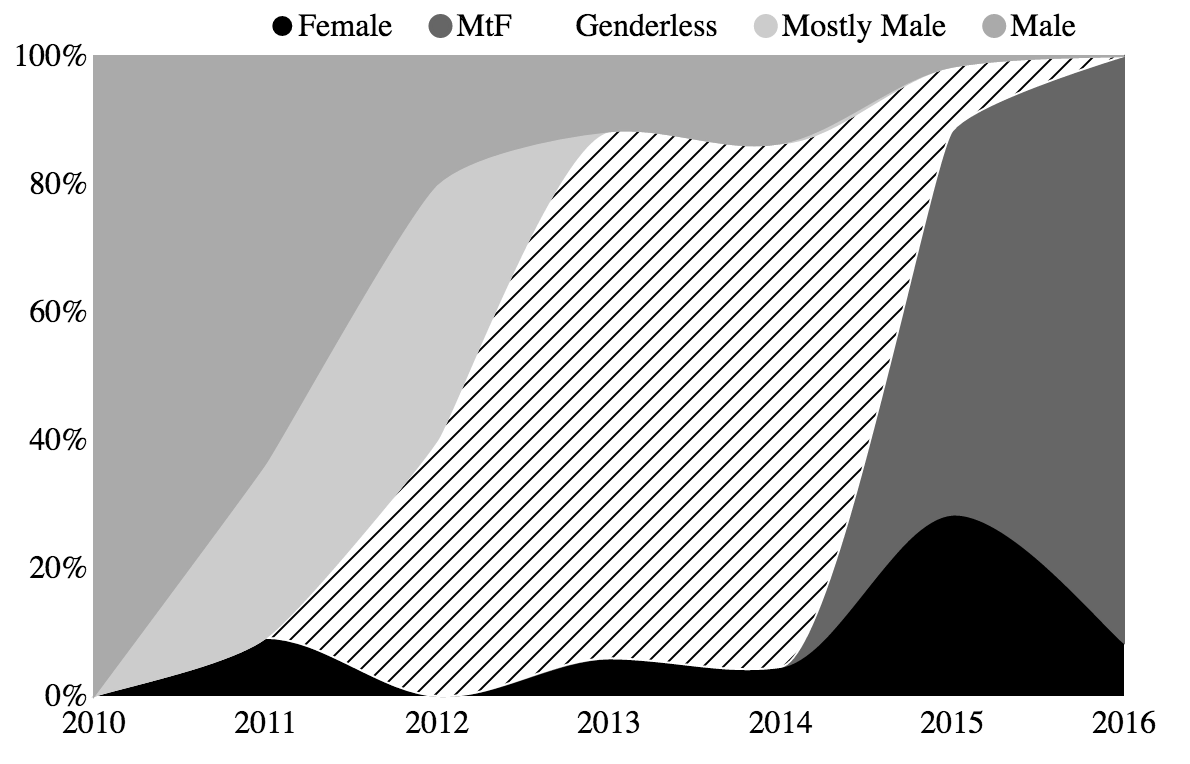
\includegraphics[scale=0.45]{assets/commissions-sex-preview.png}
  \caption{\textit{Gender expression of the author's character as portrayed in visual commissions over the years.}}
  \label{fig:commissions-sex}
\end{figure}

Figure \ref{fig:commissions-sex} shows the ways in which the sex of my characters in art that I commissioned changed over time.  There's a very clear trend from male to female, then from female (as an idealized form of myself) to a specifically trans fox (as I started to get comfortable with my identity as a transgender person).  I'm not alone in this progression, either, as many have found the utility in having a mostly safe space in which role-play is common and accepted behavior in which to explore various aspects of their identity.

There's a very good reason for this, too, but first, lets hear from another critter using furry as a lens to help in the explorations of their gender.

\secdiv

%%%%% Indi may not be able to take part
% \begin{center}
%   \textit{The intro is super rough and needs to be thoroughly reworked.}
% \end{center}
%
% Indi is many things.  We all are, of course, but ve is a wonderful example when it comes to building up the critter you want to be out of the things that are important to you.  Ve is most commonly a plush coyotter --- a coyote/otter hybrid in stuffed animal form --- covered in glowy markings in teal, purple, and green. Everything is chosen very deliberately.  Ver constituent species is each important to ver in its own way, as well as each of the colors chosen as\ldots{}tattoos?  Markings?  Shifting signifiers of emotion, attitude, and status.
%
% You see, this is why I love postfurries so much.  No other crowd that I've had the chance to spend time with has been so interested in self-actualization of so many portions of their identity.  Postfurry is a topic for another piece, but it's worth bringing up that Indi typifies the class: ve is doing ver best to find a way to not just emulate but become what ve feels verself to be, but to actually achieve that as ver reality.
%
% This naturally finds its way into the ways in which ve experiences, expresses, and talks about gender.  You've noticed the pronoun choices, surely --- ve/ver/vis --- but it's worth talking a little about how exactly Indi identifies, as well as how ve got there and how furry helped.

\secdiv

I just spent quite a few words talking about the genderful exploration of one critter and they way that it interacted with ver membership in the postfurry community, but these sentiments go far beyond just that small sector of furry.

I started a small, informal poll on twitter, and got inundated with responses.  The poll itself was simple:

\begin{quotation}
  Hi.

  Tell me about how furry helped you with figuring out your gender identity!

  Thanks.

  \textit{--- Tweet from @drab\_makyo on July 6, 2016}
\end{quotation}

The responses were overwhelmingly positive, though some had a few caveats.  Many said that the opportunity to create a character as an ideal form of themself offered them the possibility to find a way to be more true to more aspects of their identity than they might have had in the first place.  Furry, it seems, provides a constructive and creative place in order to explore.

You'll note, however, that I didn't say `safe place' above.  Many of the caveats to furry being a good place to explore gender surround the fact that, in a lot of ways, many folks who identify as trans or non-binary (as well as intersex folks) feel fetishized more often than not.  Gender, as we well know, goes far beyond just the interactions of genitalia.

Another caveat that I heard was that, although the subculture provided a healthy means to \textit{begin} exploring gender, many felt that the thing that helped them mature in their identity was seeing representation outside of the fandom, as well.  This was especially true for some of the non-binary folks that I got the chance to talk with.

There's much more that I can say on the matter of why furry might be good for exploration, and I will shortly, but first, there is far more data available than just a single twitter poll!  After all, as Executive Data Vix for [adjective][species], it's my job to administer the Furry Poll, the fandom's largest market survey, and then to go for deep dives into that giant pool of data.

To that end, I started pulling some numbers from the 2016 Furry Poll.  There were 3194 total responses to look at which were relevant to our topic at hand.  Here are the questions that we asked:

\begin{enumerate}
  \item What is your age in years?
  \item What best describes your gender identity?
  \begin{itemize}
    \item Masculine or mostly masculine
    \item Feminine or mostly feminine
    \item Other \textit{(NB: there were a series of options, including a write-in option, which, for our purposes, have been boiled down to an `other' category.)}
  \end{itemize}
  \item Does your gender identity now align with your sex as assigned at birth?
  \begin{itemize}
    \item Yes (I am cisgender)
    \item No (I am not cisgender)
    \item It's complicated (exactly what it says on the tin)
  \end{itemize}
\end{enumerate}

What all did we get?  Well, nothing too surprising, and let me explain why.

\begin{figure}
  \centering
  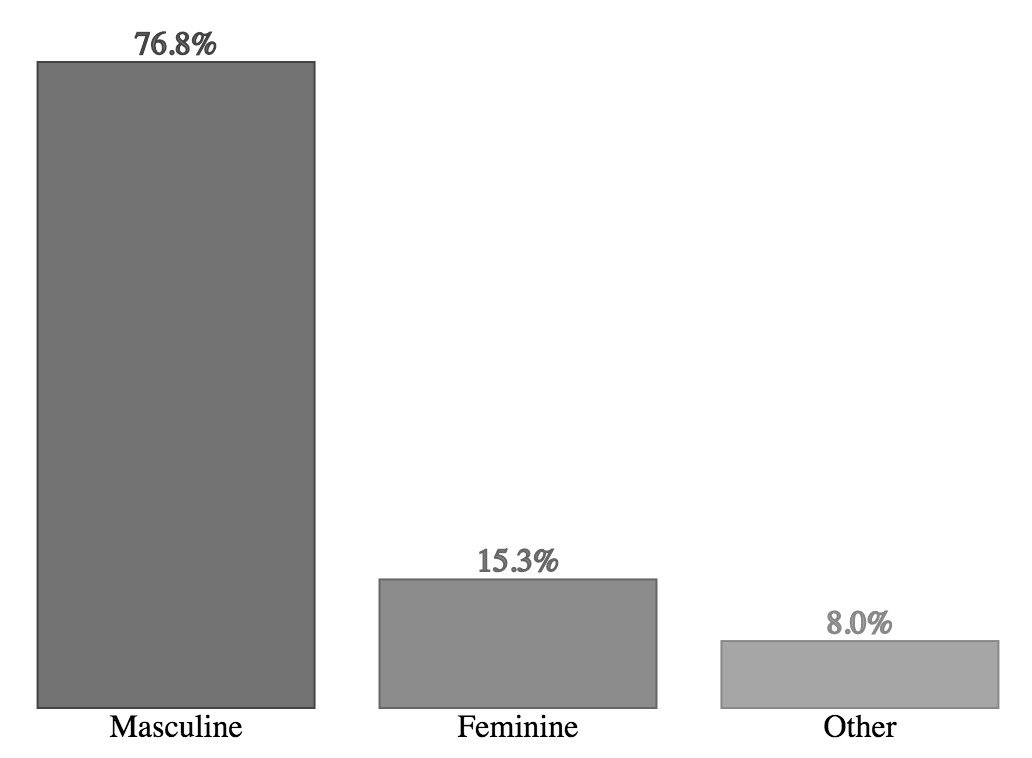
\includegraphics[scale=0.45]{assets/identity.png}
  \caption{\textit{Gender identity of respondents in the 2016 Furry Poll.}}
  \label{fig:identity}
\end{figure}

The ideas that we hold to be true without proof comprise our \textit{doxa}.  That is, the things we assume to be true, or to be the case, without needing to have anything backing those assumptions up.  When one looks around the furry fandom at time of writing, one is likely to find a subculture made up mostly of men.

To that, the survey offers only confirmation (fig. \ref{fig:identity}).  A bit more than 75\% of the respondents --- certainly a supermajority --- responded that their gender identity was masculine or mostly masculine.  Although one's expression or presentation used as a predictor has its flaws, a glance around the average convention space bears truth to this claim: we can mark that down as one point for doxa reading things correctly.

\begin{figure}
  \centering
  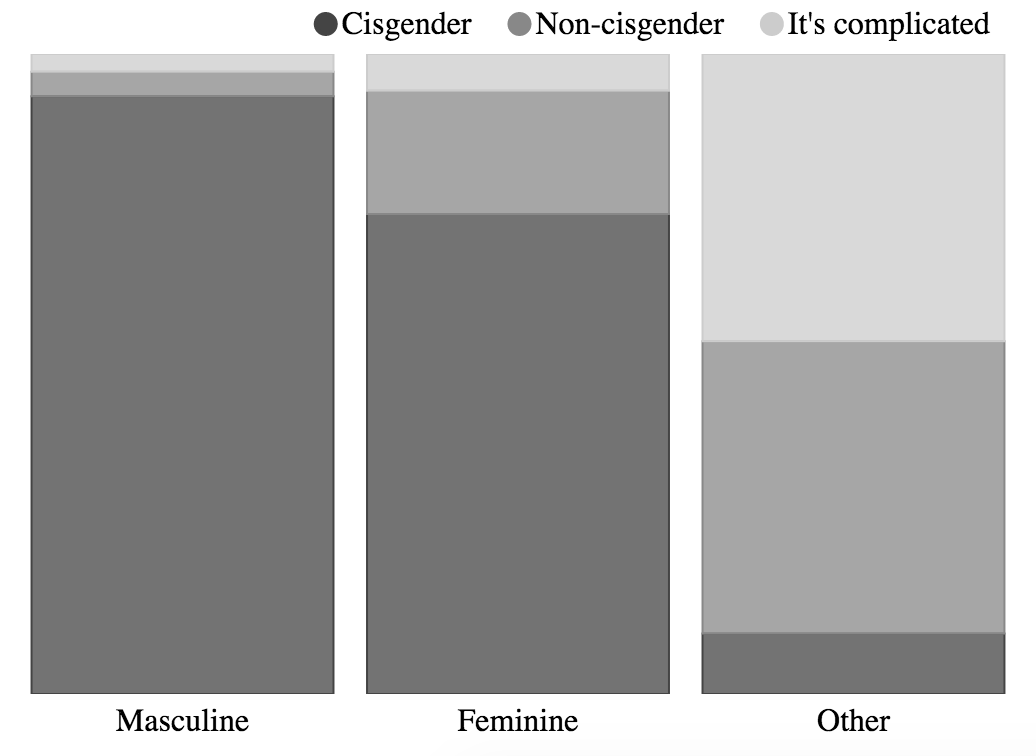
\includegraphics[scale=0.45]{assets/alignment.png}
  \caption{\textit{Gender alignment of respondents in the 2016 Furry Poll.}}
  \label{fig:alignment}
\end{figure}

Now, how about we look at gender alignment (fig. \ref{fig:alignment}); that is, let's take a look at the breakdown of how folks' gender identity aligns with their sex as assigned at birth.  For example, a trans man who was assigned female at birth, but identifies as a man now, would be someone who would fall under the umbrella term of `transgender', while a man who was assigned male at birth would fall under the term `cisgender'.  Additionally, for the sake of completeness, the survey also offered the choice for the respondent to answer that the answer was more complicated than these two choices would allow (we did not ask for further details, and had we, we would not be able to share them while preserving anonymity, of course).

\secdiv

\begin{center}
  \textit{Another story}
\end{center}

\secdiv

Given the stories of those exploring and expressing gender and identity through the framework of furry, the obvious next question that needs to be asked is ``why?''

Naturally, these sorts of things are not answered by any simple quip, nor even a single article like this.  That said, there are some things that we can point to that might help explain just why the furry subculture plays as big a role as it does in the formation of its members' identities, gender and otherwise.

There are a pair of twinned concepts within the realm of psychology that have been applied to this topic in particular.  Aaron Devor, a sociologist and dean of graduate studies at the University of Victoria in Canada, described them most succinctly in their paper, ``Witnessing and Mirroring: A Fourteen Stage Model of Transsexual Identity Formation.''

The stages themselves are interesting, of course.  They describe the path that a trans person might take as they work through the process of coming out, transitioning, and so on.  I'm not going to list them here, to save on ink --- the paper is free, easy to find legally online, and worth a read on its own.  I'd like to talk about the twinned concepts mentioned in the title instead, as they play a much more integral role when it comes to figuring out why furry might be a good place for so many to explore identity.

Witnessing is the idea that we gain something in the way of validation by having others see us as we see ourselves.  For someone who is solidifying the image of themselves as they feel others ought to see it, to have someone outside themselves perceive them along those lines is incredibly validating.  For trans women to called ma'am, or trans men to be able to use the men's room, or for non-binary folks to be referred to by their proper pronouns\ldots{}all of these things are a form of witnessing, and help to reinforce the individual's sense that they are doing what is best for their life.

To go along with that, mirroring is the idea that we gain validation by way of seeing others who are like us.  For folks in the early stages of transitioning, this comes both in the form of seeing other folks in the early stages --- the ``I can do it too'' effect --- as well as folks later on in the process --- the ``See, it can be done'' effect.  When we see something of ourselves reflected in others, it adds a bit of realism to something that might have once only been a fantasy.

Within my circle of friends, we talk of the `gender cascade'.

This goes far beyond just our little in-group.  Folks have often talked about the cascade, perhaps using terms such as `transplosion', or one news source's amusing choice of `transgender mania'.  In both cases --- either constrained by the constituents of a subculture or relatively unrestricted and part of society at large --- those who are questioning their gender, or even those who are certain but unsure of beginning transition, can gain validation through witnessing and mirroring.  That is, they can allow themselves to be seen as they are in safe contexts and see others who are like themselves in order to gain the confidence to move forward.

Furry provides fertile soil for this sort of thing due in large part to the fact that we explicitly design the image that others think of when they think of us, through the formation of our personal characters, avatars, or fursonas, however you want to think of it.

If you flip back to the graph of the sex of my characters that were represented in commissioned furry art, you can see a very definite shift away from male.  At first, I shifted from masculine to explicitly genderless, because my identity had become so painful to me that my instinct was to escape.  From there, as I gained confidence and with validation from others, I started to incorporate more and more feminine aspects into my characters.

Your character is an unspoken-yet-explicit way for a fur to say, ``This is how I ought to be seen.''  For trans folk, it provides a useful tool in terms of exploring gender identity: although mirroring becomes mudding in many circumstances (for those role-playing as a different gender, being outed as such isn't exactly desirable), it sure as hell makes witnessing easier.  I became a fox girl on the internet long before I got the letter that allowed me to start hormone replacement therapy.

There's a conclusion that I draw from all of this, though it took, me some time to connect the dots, pull it up, draw it all together, and many other metaphors.

When I started associating with animal people on the internet, I did so as a fragile teen who could barely admit that sex was a thing that existed, much less a being with a sexual orientation, never mind one that might not be straight, or even sexual.  Meeting and interacting with sexual, non-straight, and happy folk helped change that over the process of a few years, and a few halting relationships.

(Exes, if you're reading this, I don't apologize for being a gawky youth with awkward pretenses of sexuality, or for the late-night whining, but I will apologize for being a shit about the way things ended.)

Fast-forward a few years, and there I was: a mid-twenties person in the middle of an identity crisis.  What was I?  Was I nothing?  Sex was a panic-riddled minefield of unmet expectations and awkward feelings of being built wrong.  Was a I woman, with my my dreams of motherhood-but-not-fatherhood?  Was I something in between, with the fact that womanhood discomfited me in a different way than manhood?

Here, unlike with my orientation, I had enough experience to both look around me and see those going through something similar, as well as to take a step to be seen as who I felt that I might be.  I started out haltingly, and went down a few wrong paths (looking at you, plush phase; love me some plushies, but it's not me), but I found myself a niche.  It came in the form of a description and a few megabytes of graphical data culled from the minds and tablets of some artistically minded friends.  It led to me confronting my therapist one day and saying, ``Hey, can you write me a letter?''

Fast forward another year or two, and where am I?

I'm putting together the pieces of the fact that this isn't a uniquely trans thing, though this is an article on the intersection between gender and furry.  Neither is it a uniquely sexual thing, though the intersection between sex and furry is worth an article of its own.  It's something one layer up.  It's membership in a community that provides a mechanism and a place for these discoveries to take place.

Is it a uniquely furry thing?  Almost certainly not.  However, there's no doubt that furry played a rather large role in it for me, just as it did for so many other folks.

Without furry, I might just as well have come out as gay, then neutrois, then genderqueer, then trans, then all of those other wonderful labels.  But would I have felt safe doing so?  Would I have gotten all of the validation that I needed to feel healthy doing so?  Would I have come away with countless other brothers, sisters, and non-binary siblings in whom I could confide, admire, and rejoice?

I don't know.  I think not, though.
% expand this last section, ends too suddenly

  \chapter{Late August}

``Did you practice?''

Justin stared down at his dinner, a one-pot chicken and noodle dish that Jeff had perfected in the years of raising his children, spooning up small bits of chicken and ignoring most everything else.  Not their favorite, but it at least passed muster after a day of work, for Jeff, and school shopping in the evening for the kids.

``Justin, I'm not upset,'' Jeff sighed, composing himself so as to reflect that.  ``I'm just curious why you didn't get into band.''

Justin shrugged in response, his shoulders sinking lower than they had already.

``I mean, come on, man.  You don't think it's a little weird that you spend all those years focusing on this thing, and then suddenly it's just gone?''

``I tried practicing,'' Justin mumbled.

``And?''

The boy languidly picked at his dinner, found another bite of chicken, and ate that, not responding.

Jeff sighed.  ``Hey, I'm sorry, Justin.  I know the move hasn't been great for you, but you just seemed to have so much fun with band.''  He poked around in his dish, chewed a mouthful of food thoughtfully, and tried a different tack.  ``You said you tried practicing.  Just not feeling it, bud?''

Justin shook his head, bangs shifting over his brow to hide his face.  Another wan bite of chicken and more silence.

The table sat in near silence for a bit, the only sound that of Kayla poking around her empty bowl with her fork, drawing something in the cream-of-mushroom-soup gravy that was left in the dish.  A flower.  Jeff took the opportunity to clear his own plate, keeping an eye on his son, who managed at least half of his food, Jeff's measure of `at least enough'.

When Jeff finished his last bite, Kayla leapt from her seat and picked up her bowl, fork clattering against the rim.  ``All done, all done!'' she cried, trooping off to the sink to deposit her bowl there.

Jeff settled onto his elbows, leaning over the table toward Justin and lowering his head so that he could see under the boy's bangs.  ``Everything alright, kiddo?''

Justin hesitated a moment before shaking his head, ``None of it really matters, in the end, dad.''  Slowly scooting his chair back and standing up, he shuffled over to the kitchen.  He scraped the last of his food back into the pot -- it would become leftovers for lunch the next day -- and set his bowl into Kayla's.  Making his way slowly out of the kitchen, he shuffled down the hall and closed his bedroom door quietly after himself.

All that was left was the soft noise of the radio playing in the living room, where Kayla was drawing.

Jeff sat back in his chair and frowned at the bowl ahead of him.  He'd call the school tomorrow, without letting his son know, and see what was up, if his new teachers had noticed anything about how he was feeling during the day.

\secdiv

Jeff never did manage to call the school, the next morning.  He'd hit snooze on his alarm and wound up cutting breakfast time a little short.  Hustling the kids and drinking some too-hot coffee a little too fast, he'd gotten the children to their schools and made it into the office by eight, but only just.

``Perez!  Sneaking in just under the line, huh?''

Jeff whirled in the lobby of the small architectural firm, the reason he'd moved across the country in the first place.

``Mr. Pike!''  Jeff tugged his jacket straight and corrected his posture, holding out his hand to the company's owner just coming through the front door.

Mr. Pike smiled and shook Jeff's hand, then clapped his left on Jeff's shoulder.  ``Chill, Jeff, you're fine.  No need to rush.  We've got half an hour before all-hands, and as long as you're not consistently late, no one really cares.''

There was the soft sound of the doors opening behind them, and two others -- higher up in seniority than Jeff, judging by their suits -- sauntered past them and offered a greeting, ``Mr. Pike, Jeff.''

``See?  Even the boss can afford to dally in the lobby.''

Jeff smiled faintly, but nodded.  The boss's reassurances aside, he still felt compelled to make a good impression early on, especially if he planned on making a name for himself in the business down the line.

He trooped into the office after his boss, slipping out of his jacket to let it dangle from his hand.

There was still time to grab some coffee before the meeting, so, after dropping his jacket off at his desk, he made his way to the kitchen.  Whoever had gotten there before him had finished off the pot of french press, so he set about making another.  There was something comforting about the rush of warm water over his hands as he cleaned out the pot and the filter, and the simple act of scooping beans into the grinder.

It was the noise of the grinder that started to wake him up a little more, along with the smell of freshly-ground coffee wafting up to him.  He knocked the grounds into the bottom of the press and filled it with nearly-boiling water from the kettle.

The five minutes it took to brew the coffee gave Jeff plenty of time to consider the conversation the previous night.  It was too late for him to call the school, but something was clearly up with Justin.  He had been so deeply involved with music, for him to have dropped that interest completely 

  \chapter*{Chapter Three}
\addcontentsline{toc}{chapter}{Chapter Three}

As RJ slid eir hands from the pads and leaned back from the headrest, ey let out a full-fledged yawn, startling even Priscilla across the room with the sound and the stretch. Ey stumbled up out of eir seat and over toward the still-purring cat, stroking over her ears once more as she butted her head up against eir hand, eir mind whirling with a mix of work, of Cicero's disappearance, and of school with Sasha.

``I'm wiped, Prisca,'' ey informed the cat, who simply purred louder.

Smiling, ey peeled eir shirt off over eir head and slipped out of eir jeans, knowing that tomorrow's dress rehearsal would mean full dress for everyone and makeup for the actors. Ey'd have to make sure eir suit was clean, or ey'd be in trouble. For now, though, as it neared two, ey focused mostly on making sure the door was locked and the lights were out before stumbling over to bed.

As ey flipped the screen down on eir workstation to signal for it to go to sleep and wandered over to eir bed, ey couldn't get Sasha and all of her talk of high school, gone these last fifteen years now, out of eir head. Even as ey climbed into eir narrow bed and pulled the comforter over em to ward off the chill of the night, ey was replaying scenes from school, back in the US, through eir head, a worn out film, dim and scattershot, but still laced with emotion.

Ey and Sasha had tried dating early on. Later, after a few weeks of it not going anywhere, they had both admitted that they had felt pressured into having a relationship in school. Good boys and girls fell in love with other good boys and girls, pretended they didn't have sex, and went out to the movies together. They had continued the trend of going to movies, and later to live performances, together, but the relationship had petered out, rather than ending in some climactic fashion. Sasha had gone on to have a string of other relationships, some earnest and some not, some more intense than others -- a string that remained unbroken, if tonight's conversation was any clue -- but RJ had stopped there.

The social pressure to date throughout high school was only equaled in intensity by RJ's apathy toward the whole scene. Ey'd felt the occasional twinge of romantic attraction, and to other students of all genders, but the expectation of sex that went along with the idea of a relationship so put em off that ey had instead buried emself in eir school work. Ey did well in some courses and not as well in others, but on the things that ey enjoyed, ey dumped all of eir effort. Ey had gotten started early on in working the school's older sound board in their theater, running sound for plays, concerts, and assemblies, quickly earning the trust of the other tech crew and the school staff and faculty, rising to lead sound tech within a year.

Computer class had captivated em as well, and for eir sixteenth birthday, eir parents had surprised em with the implants that would be needed for full interfacing with a workstation. To be honest, it hadn't been too much of a surprise: eir father was an engineer and eir mother a fairly forward-thinking person, and they had promised em the procedure eventually.

It was a simple afair that took place in an outpatient office, involving self-guided implants that had largely installed themselves. The worst part had been the itching. It was bearable on eir hands and along eir spine, where the implants breached the surface of eir skin, because at least ey could scratch (though ey had been cautioned to try not to), but the worst had been the NFC pads in eir forehead and the interferites embedded even deeper, providing an itch that no scratching would ever reach.

Sound and the interface had taken up all of eir energy throughout school, leaving little time to worry about the social stigma that went along with not having a relationship. Ey was simply the nerdy sound kid who knew more about computers than even the teachers.

Training on the interface was a daily task that ey had applied emself to with gusto. It hadn't always been fun, of course, but by the time ey'd reached that age, ey was starting to understand the idea that work put into a craft was a good way to get more out of it. That ey had found furry around then was another thing that kept em going, working and improving at the art of interfacing with eir workstation in a way that felt natural to em and came off as natural to others on the `net. Ey moved effortlessly through the Crown Pub and a few other choice spaces, slowly crafting the primary persona that ey used when interacting with others, the cross fox known as AwDae.

It was then that ey and Sasha had really started connecting, for it was her that introduced em to the community. They started hanging out more, talking more, and, especially, building a network of friends together. Dating hadn't worked out for them, what with RJ slowly coming into eir identity as asexual and more and more androgynous over the years, while Sasha remained fairly sexual and interested in guys much more masculine than em. All the same friendship had seemed almost natural.

The training had culminated in an offer to go into interactive sound technology at a rather prestigious university out on the east coast. It meant leaving Sasha and a few other close friends behind along with eir family, but it also meant that ey would be at the forefront of a new technology used in production of both films and live work. In fact, the field was so new that eir own studies at the university helped fuel the change in theater tech work, eir dissertation, what was meant to be eir capstone project, being eventually published and spread around the world.

Ey had continued to work at the university for a while, as they were one of the few places around with both a theater and the technology to back it up in such a way that ey had helped create. Ey had considered continuing eir studies beyond where ey had, but the draw of the theater was what focused em most, rather than strictly academia, or even limiting emself to college theater.

The call from London, had come less than a year after ey graduated. Would ey like to help start a tech-savvy theater group in town? The pay would be slow to start, but the troupe had a loose collection of apartments ey could stay in. Ey would have full run of the sound department. When could ey start?

That conversation had taken some convincing, when it came to eir parents. They were pleased, to be sure, but they also felt that London was fairly far away, even though still in the western bloc. Ey made eir promises that ey'd come and visit every now and then between shows or when an understudy would take a show for em.

Burying emself deeper into the covers and the mattress, leaving enough room for Priscilla to join em later, RJ thought more about what had come up between em and Sasha before. When they'd Lost Cicero, it was a blow to them all. Getting Lost was not something that happened often, only a couple dozen recorded cases to date, but among those who were counted among the Lost, a disproportionate amount of them were those who were heavy users of the integration technology. It was a risk, everyone had assumed, just as was travel. Something could always happen.

All the same, it was an intense sensation to feel it hit so close to home, and it reminded RJ of just how much ey relied on the integration technology, not only for work, but for a large part of eir social life. Ey enjoyed the company of the troupe just fine, and often accompanied them out for drinks and the like, but eir heart truly lay among the friends ey'd made on the `net. His friends being on the `net meant more use of eir contacts, and more use of eir contacts meant more risk.

It was risk for all of them.

  \chapter*{Chapter Four}
\addcontentsline{toc}{chapter}{Chapter Four}

Doctor Carter Ramirez rubbed her face into her hands, ground her palms against her eyes until she saw stars, before finally slicking her hair back.  She had put it up into a bun earlier that day, but there were plenty of flyaway hairs, as there always were.

She felt out of her league.  Everyone did, here on her team, but that didn't stop the fact from wearing on her.  It's not that there was no support from on high to help with the Lost, because there was.  It's not that there was no one else trying, because there was there, too.  It's that no one seemed to take it all that seriously.  It was a thing like addiction, or plane crashes, or suicide.  Something to look at, to study long enough to say ``Ah, \textit{this} is happening now,'' and then set aside like some work of art which was only good enough to be a conversation piece.

People admitted that the phenomenon of getting Lost was happening, but only in as much as it didn't affect that many people.  A simple number to point to.

She wasn't the last one left in the lab, by any stretch, but it had reached that point of the night where collaboration had stopped and everyone was butting their head against their own individual problems, toiling in silence.  She put down her tablet and pressed down the display on the workstation that she had been assigned for this project, sending it to sleep.  It had also clearly reached the point of the night where she wouldn't be getting anything else done.

It was as though the brains of the Lost were just elsewhere, just dreaming on some level, but there was no sense to it, no rhyme or reason to why such a thing would happen to the patient.  Some of her team were working on pulling together all of the facts about the population that they could, from demographics to physical stature, searching for clues.  The neuroscientists were digging into what was going on within the brain, and what few scans they had from before someone had gotten Lost.  Their two pet lawyers (actually just law students on internship, also versed in stats) were digging into both the legal status of the Lost as well as doing what they could to procure under health information law from patient medical histories.

And Carter was supposed to tie it together.

Or, that was her stated goal.  The university medical center had grudgingly provided space and funding for the project in an attempt to win some much-needed kudos, but she was starting to doubt just how much the UMC even wanted her to continue.  As manager, she had been met with hurdle after hurdle in trying to make any progress in the case as soon as she started to venture outwards.  Colleagues assured her that all projects worked this way, but it was as though the advisory board had given her all the data that it was willing to give, and any more might put those kudos it was receiving at risk.

Carter patted her associate on the neurchem team on the shoulder and stood up, stretching her back.  ``Sorry, Sanders.  I'm done in.  Catch you in the morning?''

``Mm,'' Sanders replied, rubbing at his eyes and stretching his hands out, alternating between clenching them into fists and flexing his fingers out wide.  ``Sounds good, Ramirez.  Catch you then.''

Carter gathered up her coat and her messenger bag, taking one last look around the workstation lab, counting heads to see who would be staying later than her.  She swiped her way out of the wing so as not to set off any alarms and signed out at the front desk before making her way out into the night, bundling herself up in her coat.

At home, she scoured the fridge for a bite to eat -- she had ordered dinner for the lab earlier, but it was getting on midnight and she didn't want to go to bed on an empty stomach.  She settled on a few pieces of salami stacked onto a couple of crackers, enough to keep her empty stomach from complaining through the night and sat herself down on the couch in the shared living room.  She left the lights off so that she wouldn't bother her flatmates, or so she told herself.  In truth, the darkness felt good.  She could keep her eyes open and not be greeted with a tablet, a screen, a simulation.

She sat long after finishing her snack, listening to her flatmates sleep, thinking in the dark of all the administrivia that surrounded her task and just how she would be able to get what she needed.

Eventually, finding herself at just as much of a dead end as she had at work, Carter stood and ambled into her room.  It was small, but clean, and it served her well.  She changed from her work clothes into a comfortable pair of lounge pants and a night shirt before crawling into bed.

\secdiv

The morning's alarm startled her awake.  She had thought that the end of grad school had meant the end of six-hour nights of sleep, but apparently, that had not been the case.

Blearily, she pawed at her phone until she managed to swipe in the right direction to turn the alarm off.  It was tempting to go back to bed -- after all, the Lost weren't going anywhere, she mused -- but she managed to at least kick her feet out from under the covers and sit up.  in bed, letting her frizzed hair hang down around her face and shield her from the world for just a little bit longer.

It was her phone, as always, that brought her back to reality.  It's mere presence, even silent as it was, was enough to draw her back into the problem at hand.

\begin{quotation}
  Ramirez

  Another, this time with scans from before the incident.  Another furry, you don't think that's got to do with it, do you :p

  S
\end{quotation}

The brief message from her colleague left her puzzled until she'd put it together that he was talking about one of the other subjects' past records, indicating him as a member of a fandom.  Sanders didn't honestly believe that people who pretended to be animals on the `net were more predisposed to get Lost than anyone else.  And, to be honest, neither did Carter, even after giving it the token consideration.

All the same, the thought stuck with her through her two cups of coffee that morning, the first in the kitchen and the second out of a travel mug on the L as she headed out towards the UIC campus.  \textit{Another furry, you don't think that's got to do with it}.

She felt sluggish, and craved another cup of coffee even after she'd reached the bottom of the mug she had with her.  The thought nagged at her, caught like some spinning shape against the threads of her thought in a way that the rattle and screech of the train couldn't displace.  It tugged those threads free, stitch by stitch, until it reached\ldots{}what?

Until it reached the hem, and then the same thing over again.

``Holy\ldots{}holy shit.  Holy shit.'' Carter said, startling the elderly lady next to her.  She murmured an apology and fished her phone out, thumbing in a quick message to the team.

  \chapter*{Chapter Five}
\addcontentsline{toc}{chapter}{Chapter Five}

RJ allowed himself to sleep in until nearing 11 that morning, given that tonight was the last night of dress rehearsals.  Many other members of the troupe held part time jobs during the day, and he had been known to offer his services as consultant during times like these.  Even so, with all that he did, he made enough to not have to worry about holding down more than the one job

As it was, on days when they had nighttime rehearsals, he felt no compunctions about sleeping in.  There was nothing to be up for, and with only the `net to keep him occupied in the mornings, he felt little need to get moving.

It was Priscilla who has woken him up, butting her head against his cheek and purring loudly to him.  The more insistent the cat got, the less he was able to ignore her intrusions on his admittedly banal dreams.

He finally trudged out of bed and refilled his cat's water and food dishes, giving her the requisite morning pets to keep her happy.  That done, he scooped her litter box and made himself a pot of tea.  He sat at the tiny kitchen table, sipping from his oversized mug and watching the late morning traffic from his window, primarily composed of business traffic, with the occasional mother with child in tow.

% Stops for food, thinks of Cicero and checks on contacts from cards

% Heads to theater

% First half of the night goes smoothly

% First notices that the room feels smaller, then less responsive to control, then silent; finally tries to pull back and winds up just looking up from a board at his HS auditorium


  \part{}

  \chapter{Halloween}

\begin{itshape}
  Just as before, they called him on his cell phone at work.  This was the county coroner's office, and could he please come down sometime today before 5:30 to help identify a body.  Yes, now would be fine.  The sooner the better.  Thanks.

  Just as before, his heart seemed to seize within his chest.  He had taken the time to only dash off a quick email to his boss.  There was an emergency.  Yes, he'd make up the time later.

  Just as before, he left his coat slung over the back of his chair and his computer logged in and unlocked.  He jogged to the elevator, punching in the address that he had been given on his phone, but by the time he had made his way from the sixth to the first floor, the anxiety had welled within him such that he sprinted from the building to his truck.

  Just as before, he was met with calm professionalism at the door and quietly, efficiently ushered from the entrance to the room where he would view the deceased.  No, they could not tell him more.  He would have to wait, then speak with the coroner directly.

  Just as before, Karen, unmistakable as ever, lay on a clinically cold table, eyes shut, though her nose and jaw were badly disfigured from the car accident, lacerations covering her torso down to her midriff, an ankle oddly angled.

  Just as before, he knew her immediately.

  Just as before, he ran to her, the shout of anguish already welling up within his chest.

  And then he hit a wall.  There was no rebound, no noise, nothing to see.  He was simply stopped five or so feet from his wife as she lay on the table.  He could not go closer, he strained ineffectually, his muscles seeming to go slack as they encountered the transparent barrier before him, not allowing him to go to his wife.

  And the coroner's assistant or whomever had guided him there kept asking, ``Sir?  Is this your wife?  Sir?  Sir?  I need to know if this is your wife.  Sir.''
\end{itshape}

Jeff didn't awake with a gasp, though he did start enough that he felt disoriented as his eyes struggled to make out the darkness of the room surrounding him.  And yet, as the disorentation passed, he felt himself completely awake, as though he had simply never been asleep.

He rolled onto his other side and peered at the glow of the numbers on the clock, willing them to swim into focus.

\textit{Three AM.  Shit.}

It was that awkward period of the night where he knew that, unless he got to sleep immediately, there would be no making up for the lost rest and he would feel terrible all day.  And there was no way he could sleep soon.

The pain of losing Karen had slowly left him over the months and years that followed her death, and love for his children had taken over once the estate had been settled and life insurance worked out.  Even so, it was possible to bring back that ache with a simple memory, or a dream.

  \chapter{Early November}

``Oh!  Kayla!  Those are beautiful!''

Kayla looked up, dully at first, from the crocus she had been drawing, one among many, in a sea of graphite.  Recognizing the voice as Mrs. Willis, she had brightened and smiled, setting her pencil down and shuffling the papers nervously.

``You think so, Mrs. W?''

Mrs. Willis beamed down to Kayla.  ``They're beautiful, dear.  Where did you learn to draw like that?''

Kayla shrugged, her feet swinging, crossed at the ankles, beneath her chair.  ``I just draw a lot.  Daddy draws, and so I started drawing, and now it's just what I love to do.''

``They're beautiful,'' Mrs. Willis reaffirmed, then paused.  ``The class is scheduled to move to clay tomorrow.  Do you want to work with clay?  I can let you do clay flowers, if that's what you like, instead of the slab pottery.''

Kayla, thought about that.  The thoughts were crowded with flowers.  Perfect curves along petals, the gentle arc of a stem softened by trichomes.  Colors that seemed to blur within her head.

``I-'' she began, then stopped once more.

Perhaps sensing the remainder of the thought, Mrs. Willis took stock of the rest of the class, drawing inverted images as a study of negative space, though she hadn't introduced that term yet.  Other than a young boy and girl trying desparately not to look like they were talking across the room, everyone was behaving well.

``Come, Kayla.  Come with me.  I want to have a word with you in the hall,'' she murmured quietly.

Kayla flushed, gave one last look to her flowers, and nodded, carefully scooting her chair back from the edge of the desk.  She followed after her teacher, mindful lifting her feet too high.  It was best to move among flowers in a flowing fashion, with grace so as not to crush any.

Once outside, Mrs. Willis closed the door most of the way after one last look, then appraised her student.  ``Do you know what an `independent study' is, Ms. Perez-Gray?''

Kayla stared at her feet (surrounded by dandelions -- delicate flowers of all yellow on a sturdy stalk) until the words `independent study' caught her attention.  ``Mmn?  No.''

``It means that a student gets to direct their own study into a field that they love.''  Mrs. Willis peered down through her glasses at the young girl, ``You have an interest -- a thing that you love -- and you have the will to make something beautiful.  Would you like to do an independent study?''

Kayla poked her toe against the linoleum (against the green leaves at the base of a dandelion) and thought for a moment, ``What does that mean?''

Mrs. Willis face softened into kindness.  ``It means that I would give you resources to learn how to draw and paint flowers.  Some books, some examples.  Georgia O'Keefe\ldots{}no, not yet.  Anyway, dear, I'll give you some examples and books on drawing flowers, and you and I will come up with some goals for you to reach, and you can work towards that, rather than following the curriculum of the rest of the class.  Does that make sense to you, Ms. Perez-Gray?''

The flowers were so fragrant.  They smelled like muffins.  The color drained from them down into the linoleum, then flowed back into them from the ceiling.  Yellow and green -- gray -- yellow and green.

Kayla nodded.

``Good.''  Mrs. Willis smiled brightly.  ``I'll write your father a note during class today.  You can bring it to him and it will explain what we plan on doing.  I'll leave a spot for a signature at the bottom so that you can have him sign it.  Bring it back to me, okay Kayla?  So that I know he's alright with our little plan.''

Kayla felt neither relief nor upset, nor anything really.  She was overwhelmed by the heady scent of a field of dandelions, coarsely toothed leaves brushing against her ankles and reminding her that this was good, that this was right.

``I will, Mrs. W.''  She smiled at the tickling of the leaves against her, the sensation seeming to pass through her socks and sneakers.  ``I will.  Thank you, Mrs. W.  I want to draw more.''

  \chapter*{Chapter Three}
\addcontentsline{toc}{chapter}{Chapter Three}

Carter had come up against a unique hurdle.

One of the problems with the genderqueer patient, RJ, was that, although it was notionally feasible for em to have an X in their gender records and all the pronouns ey chose, not everyone had recognized that.  Various pronouns flourished and died, styles of dress had come and gone, but the arcane triad of institutions -- banking, health care, and government -- remaned stodgy and stuck in their ways.

As a result, RJ existed in a unique limbo in some cases.  Although eir passport specified X under the gender marker, although ey went by eir own pronouns (which, Carter was informed, were a truncated version of singular-they known as Spivak pronouns or Elverson pronouns, depending on the source), and although ey functionally lived life as a genderqueer person, without close ties to anyone, ey still had records that marked em as male in the arcane triad.

This, by itself, was not an interesting fact.  Even though folks had been doing similar for going on centuries now, there were still articles and posts about the perceived barriers to entry when interacting with the world as a genderqueer person.  Person after person had complained about the difficulties in changing one's gender marker -- a letter from so-and-so, such-and-such documentation -- and person after person was turned down by clerks of the court for various reasons; take your pick of: ``we don't do that here,'' ``you have to do that at the federation level,'' or ``you'll also need this [unrelated document]'', among countless others.

Everyone had imagined, as medical technology had advanced around the subject of gender, that such changes would become easier as the world moved on past gender.  Some held decidedly more dire predictions in their heads than others, of course.  It hadn't quite worked that way, though.  The fractious nature of identity combined with regime shifts had left quite a large gap for people to fall into.  Nearly a hundred years after transgender rights had been codified, there still existed only the M, the F, and the X.

What Carter was learning was that the X came with a whole bouquet of baggage.

Before one grew up and settled on an identity, one was burdened with either an M or an F on official paperwork; this despite years and decades of campaigning.  The result was, as far as she could tell, a duplication of records.  One wound up with an M or F record that was linked permanently to one's X record.

Carter had only the faintest idea of why it would be so difficult to change records unilaterally.  Having worked for her fair share of time in academia, she had become inured to the committee culture of university life.  Government, she supposed, was like university, only hundreds or thousands of times the size.  Rather than one single database storing individuals embedded within a system -- citizens, that is -- there were likely countless such databases.  Updating one's gender record caused a ripple that propagated through databases in a way that was understood by the makers at the time, but `at the time' often referred to a time when legislation was passed.

The result was that Carter was coming across two records.  There was RJ (X) and RJ (M).

Oh, rather, Avery Croft, her subordinate in the stats and history department, had come across this problem and eventually kicked it up to Sandra, their lawyer.  Finding no clear path forward that could be found under a ten percent time bargain, Sandra had kicked it further up the ladder, and now Carter was dealing with the multiplication of records.

\textit{That's okay,} she thought to herself.  \textit{This is my job.  I'm the one who ties things together, and this is just another one of those.}

She was parked before three decks, delved into her workstation.  She had a deck for RJ (X) of pretty substantial size, a deck for RJ (M) of much smaller size (some of which was, doubtless, duplicated in the first deck), and a deck that she was working on, titled simply `research'.

To her right were two additional decks.  One for Cicero (M) and `research'.  Cicero (M) was an enormous deck.  Even among the countless decks of cards scattered through the shared system that the team was using, it was among the largest.  Cicero had more than just a little bit of past behind him, documented through various channels.

Were Carter to zoom in on Cicero's deck, she knew she would find thousands, perhaps even tens or hundreds of thousands of cards detailing interactions with the DDR.  These were `paperclipped' together, a shorthand to say stuffed in a folder without being separated from the rest of the deck, such that, by leafing through the deck, she simply came across one large entry encompassing all its component entries: a grouping within a grouping.

From what she could tell, however, skimming through the `research' deck, was that the two had encountered very different sorts of interactions on the `net, even taking into account their varied interests.

Collin Jackson was almost a parody of DDR addict, whereas RJ Brewster was a quiet, introverted person online, choosing to interact, when ey interacted in public, on a one-on-one scale.  However, they were both solid participants in the furry subculture.

% the thing is that RJ's unique position as an outlier gives the team more insight into actual problems: ey's slipped through a lot of automated checks based on outdated assumptions of gender

  \chapter*{Chapter Four}
\addcontentsline{toc}{chapter}{Chapter Four}

It took AwDae just under two hours to find the microphone.

The first hour was spent searching the auditorium thoroughly. Ey searched by walking around clapping and humming, then singing songs half-remembered from productions ey had helped with in the past. Ey would've whistled if it wasn't for the structure of a canid muzzle. There was no way eir lips would manage to pull that off.

Silence.

After an hour, venturing even into the overhead areas where sound wouldn't reach, ey gave up and took a break.

Taking the slip of paper with Cicero's transactions from eir pocket once more, ey scanned over the titles of the initiatives voted on. There was very little there to latch onto. Or, rather, there was way too much. AwDae couldn't manage to even boil down the table into any single sentence, much less something useful. The cat had apparently voted on just about everything, without taking any breaks.

Eventually, when the rows started to blur into one another, ey levered emself up from the auditorium seat ey had chosen. Ey refolded the paper and slipped it back into the pocket before checking on the board once more. Everything remained set as it was before the break.

Venturing outside the auditorium, AwDae had imagined ey would work in concentric circle away from the auditorium. This turned out not to be the best idea. The theater was nestled between two arms of the school which did not meet. That made their routine fairly artuous. Ey'd walk down one hallway, poke into classrooms, and make noise before moving on. When ey reached the end of eir circle, ey had to jog around the auditorium through the student center to go down the other hallway and do the same

Eventually ey gave up on the concentric circle plan and started working from north to south.  Ey worked through the entirety of one hallway, clapping and hollering, without hearing anything, before moving on to the area of the student center near the auditorium.

It was there that ey heard the first, faint hum.

At first, it had skimmed beneath eir attention, sounding rather like an echo from eir own voice in the cavernous space of the student center. When the open doors to the aduditorium caught eir eyes, ey tried once more, getting another faint hum that slowly died out as the space and air dissipated the tone.

It took another few minutes to find the microphone itself: a small bit of hardware resting delicately atop the door handle leading into the principal's office just to the northeast of the auditorium doors. It was surprising, in a way, that ey hadn't managed to trigger any feedback earlier, until ey realized eir mistake: ey would have to shout loud enough to be heard in the auditorium; without the speakers producing noise loud enough to make it back through the walls and reach the mic, there would be no feedback.

The door was labeled `Admin.', which was omminous. Although there was a head office at the front of the school, administration was where the principal and vice principals' offices were. It was one of those places that lingered in the mind of every student who had passed through the doors of the school. Getting called to the front office was usually bad enough -- a call from a parent!? -- but getting called to the admin office was worse still.

AwDae delicately picked up the microphone through mounting feedback before shutting it off, eir ears laid flat in an attempt to shut off the growing hum from the auditorium. The sound stopped a scant few moments after the mic was shut off, bouncing around the auditorium and the student center.

Ey pocketed the mic in eir trouser pockets and straightened back up, cautiously lifting eir ears once more. The school was once again silent. There was no hearing the hiss from out here in the student center. Remembering the position of the mic, AwDae wandered back over to the auditorium, turning the gain back down on the board and lowering the house volume. Ey even turned the mic back on and gave it a quick ``one-two'' to ensure that none of the speakers had been damaged.

\textit{This is a sim, and not even mine,} ey thought, ears tinted pink with a blush. \textit{What does it matter if a speaker blew?}

Ey shrugged it off after a moment. Habits were habits and there was no reason to break them now.

Wandering back to the admin office, tail swishing behind em, AwDae couldn't help but feel as though ey was trapped within a game, one of those first-person puzzle solvers that seemed to be forever popular. The fact that ey seemed to be receiving what amounted to clues while in an complex abandoned building only added to that.

Shaking eir head, ey turned the knob on the admin office and peeked carefully inside.

There were no traps, no jump-scares, just the six-sided room with its three doors on the opposite walls. One for the principal, and two for the vice principals. Taking the game metaphor to heart, ey started poking around the office where ey could, flipping through a datebook on the secretary's desk (empty) and rummaging through the drawers (office supplies). The waste baskets were empty.

Steeling emself for something shocking, with the game mentality still holding onto eir mind, ey tried each of the doors in turn.

It surprised AwDae that it wasn't the principal's office that opened, but one of the vice principals, though the name escaped em. The office was dark, but the lights responded to a touch on the pad, which ey sent to a comfortable level without being intimidating. Ey remembered being hauled into the room, all those years ago, with the lights all the way up, a gesture of power.

Rummaging through the desk revealed little of note. Rather than a planner on the desk, however, was a workstation; simple and, to eir eyes, ancient. It didn't respond to any of AwDae's interactions, though. Although how it would work, ey didn't know, ey had hoped that a connection like that might lead to a way back out of this mess.

The only other item on the desk was a scratch pad, and a pencil. They never seemed to go out of style. The pad contained a simple breakdown of costs, divided into departments, for the coming year. A simple three-column setup tallying subject, expense, and deductions from some number at the top which must be the classroom budgets. At the bottom of the page, was a final number, circled. Apparently, the administrator hadn't quite liked the result, for it was circled in dark, angry strokes.

AwDae flumped down in the chair at a bit of an angle, letting eir tail flop down between the arm rest and the chair's back so as to keep from crimping up uncomfortably. Tired, so very tired.

Ey rubbed eir eyes tiredly, brushing away the sandy grit of tears already shed. Ey was moving in this search with determination, occupying eir mind, specifically so that ey wouldn't collapse into a depression borne of hopelessness and despair. It occurred to em that getting Lost was the perfect prison: complete freedom, or nearly so (ey had already fantasized about jimmying open the other doors), with nothing to do. Nothing to dream, nowhere to go, nothing to know.

Ey would go mad without a task. Ey could create, but why create in these empty halls? What would ey even begin to create that would matter the worth of a damn? Ey would never be able to share it. Ey would only be able to spiral inwards. Endlessly.

All AwDae wanted to do was curl up in the chair. It was comfortable enough, ey could probably manage to get some sleep in.

Instead, ey rubbed eir eyes once more and leaned forward toward the desk, letting eir eyes focus on the columns of scratched digits and marks on the sheet of scrap before em. Mindlessly working through the sums in eir head simply for lack of anything else to do.

``Hmm, that's weird,'' ey murmured sleepily out of the corner of eir muzzle.

The numbers didn't add up. In fact, everything added up within its own row, it was simply as though a row were missing.

Ey yawned and stretched before holding the sheet of scrap up to the light. There were no erasures, whiteouts, or anything like that. There was just simply not enough information.

Finally, the fact that ey was holding onto a ledger, such as it was, dawned on AwDae. If ey was meant to be looking for clues, then\ldots{}

Ey hastily fished the previous clue out of eir pocket. The ledger of Cicero's DDR interactions.

It wasn't nearly so simple as the scratch paper. For instance, each referendum had three different types of interaction: a cost, a bounty (if that referendum was referred back to the house), and any number of comments made on the issue, and they were often out of order on the sheet, given Cicero's habit of voting on everything.

Ey wished for eir workstation more than anything, as this would make the task almost trivial. Having to do without, ey snagged the half-used pencil and the rest of the scrap and worked it out. Each cost and comment would be a debit, and each bounty would be a credit. One could also buy DDR credits through a mechanism that basically acted as an additional withholding on one's taxes, and there were two of those in there, ensuring that Cicero would have enough DDR credit to make what AwDae assumed was some scathing political rant on an upcoming high-stakes referendum.

Even so, with all that work, it was clear that even the section of numbers on the paper didn't add up. Once more, there was a missing interaction. Three missing interactions, rather: one vote's cost, one vote's comment, and one vote's bounty, at AwDae's best guess.

The problem was that one's DDR records were public -- they had to be, for the system to work -- and, unless it had been tampered with (something AwDae had to take into account), eir was a combination of 1,252,000 credits unaccounted for in terms of transactions. One million debit to the comment, a quarter of a million credit for bounty, and two thousand to the vote cost.

AwDae tore off the top sheet of scrap and, working faster this time, ran the numbers once more, only to receive the same result.

``Well, huh.'' Ey sat, stunned, for a little while longer before gathering eir notes and folding them together with the original clue and stuffing them into eir pocket. Ey couldn't create a deck here, but ey could sure take items with emself.

If this all had something to do with what was going on outside, where ey was counted among the Lost, that was all well and good. But, how would ey get that information back out.

It was probably too early to be thinking of such things. Ey wasn't going anywhere for the time being. Sleep was taking too strong a hold on em. Ey gave token consideration to where ey would be able to sleep before deciding on the auditorium. The fold-down seats were cushioned, but not very well. All the same, the place had a sense of home about it. Perhaps the day to come would help em learn more.

  \chapter*{Chapter Five}
\addcontentsline{toc}{chapter}{Chapter Five}

Carter hadn't meant to dodge her subordinate's question.  They truly did need to go in to eat.

The food was, as promised, delightful, and Carter made a mental note to come here more often for more good Vietnamese food.  That note, however, was filed by her mind and set aside so that she could work through the implications of what had been spilled to her by the tabloid.

She couldn't visit this RJ any more than she could fly out of the second story window here and back to her lab.  There were several factors keeping her from doing so.

First, and foremost, it was useless.  Her team didn't \textit{need} access to the Lost to do all of their work, because much of their vitals was provided as a real-time stream of data into the work group.  Besides, it had been proven that physical contact registered little, if at all, to the Lost.

Secondly, there would be people between her and RJ.  Not just doctors and nurses, but her own administration.  She would have to go through any number of people just to get access to some variables that likely wouldn't help her investigation at all, such as eye color or hair color.

Finally, there was the law.  Carter understood the purpose of WFPHIPA: the Western Federation Personal Health Information Protection Act.  Hell, she had voted on it, herself.  It was something she felt strongly about.  The tabloid had technically breached that (though there was no culpability) by informing her that there was a good chance that one of the group they were studying was this RJ.

There was, however, nothing to stop her from going to a show in the next day or two.

Feeling very much the sleuth, she stuffed a small egg roll into her mouth with delight, savoring the taste of it.

Yes, she'd go to a show up in Soho.

\secdiv

With her resolution planted firmly within her, she found it much harder to make it through the rest of the day.  Rather than wrangle the two competing strands of the work group into some cohesive goal, she spent much of her time distracted.  She was thinking about all of the ways in which she could possibly approach the cast or crew.  Would she be able to even get in contact with any of them?  Supposing she would, what would she even say?  ``Tell me about your sound tech''?

Eventually, though, the rush had worn off.  Toward the end of lunch, she had purchased tickets (at no small cost) and been hyped up about visiting the theater.  When the afternoon started to wear on, she found herself once more tied up in work.

Avery and Prakash had both settled into the routine of investigating what had gone on before the incidences of the Lost.  Avery was collating what data they had from each case on the social front before the subject had gotten lost and searching for social connections between each of the cases.  Prakash, meanwhile, was digging through biochemical data that had been collected from each of the patients and searching for similarities for them, based specifically on the time before they had gotten lost, rather than during or after.

Carter had supposed that this would be innocuous enough, but it seemed that Sanders had taken the opportunity of the boss dining out for lunch to chat with a few of the other members of the workgroup.  Not once, but twice while she was working, she had fielded private messages from some of her teammates.  Both had concerns around the direction of the project, and questions about the wisdom of separating the work group into smaller groups.

In both cases, she reiterated that this would be another temporary investigation.  If it turned up any useful information, then they would have that conversation again in the near future.  If it didn't, then everyone would cohere once again afterwards.  There was comfort in the worlds, but all the same, Carter wasn't sure how much effect they were having.

She had an idea, one she thought worth investigating.  Sanders, however, had an ideal.

Or so Carter was assuming.  When assessing the team's standing on the issue, she had used a simple three point scale: for, neutral, or against.  What she hadn't asked was, in the common usage, how many fucks each of them gave.  There were, after all, two parts to making a decision.  Which way you'd vote, and how much you cared about that.

Carter could easily estimate Sanders giving ten out of ten fucks against this current plan of dividing the team for exploratory purposes.  In fact, until this afternoon, she would only likely have given seven or eight fucks.

That question hadn't been asked, though.

This afternoon, it was the combination of determination to see if she could learn more for the project and the sense that she was on the right path that had bumped her up on the number of fucks she gave.  And, if she was honest to herself, the hope of proving Sanders wrong.  There was no small amount of competition within academia, after all.

\secdiv

The play was a contemporary piece called The Short Trip.  According to the season, it chronicled an indecisive youth taking a small trip away from his family on false pretenses to visit a bunch of friends for three days.  The goal of the trip was to visit his long-distance partner, but in the setting of a party, with guests, both known and unknown, weaving their way through the scene over the three heady days.

This much she had learned as she made her way southwest.  Carter had needed to duck out of work earlier than usual to make it over to the theater on time.  She had actually to travel past RJ in the UCH, riding along the yowling Victoria line, to get to Soho where the theater was.  Traffic at that time was was notorious for keeping the Tube cluttered and, at times, inaccessible.  She had needed to wait for three trains to pass before she found one with room.

The train vomited her out into Oxford Circus and left her spinning, looking for the right exit to the tube station, each helpfully lit up with a thin, translucent display that overlaid the older signage in painted tile.  Both bore the unerring curves of Helvetica, perpetual winner of the font wars.

It was easy enough to find the theater by following the crowds, and her identity -- and thus her ticket -- was proved by a taking her glove off and giving touch from her contacts, a grip around a simple bar in front of the theater.  Once she had done so, the bar flipped around to provide its other end to the next customer, the end she had touched getting a quick sanitization so that everyone touched a sanitary surface.  It was all rather like getting on the Tube, only much slower.

Carter was surprised by just how much she enjoyed the play.  She had decided not to approach cast or crew beforehand.  This had initially worried her, as she suspected she would spend the entirety of the play thinking about what to say.  She wound up getting engrossed in the play, watching as the lead made his way through the party and met up with his partner.

The cast did a magnificent job of portraying the awkwardness of meeting up for the first time.  She had had her own long-distance fling while an undergrad, and she knew that feeling well.  Her mother had even cautioned her to meet up at a public space where you know people, like a party, just in case.

It was well into the third act of three that she realized she hadn't given attention to the sound of the play.  A passing thought informed her that this was probably a good thing, that this was the sign of a job well done.

She applauded as heartily as the rest of her fellow audience members, clapping in that way that prevented any knocking of her contacts against each other.  All the same, her mission, such as it was, was not lost on her.  She was perhaps a little rude in her haste in making her way out into the lobby of the theater where some of the cast and the director were greeting the audience.  It was opening night, after all.

``Mr. Johansson.  Mr. Johansson!''

The bulky man turned toward her with a pleasant look despite the obvious worry lining his face.  ``Ma'am.  I trust you enjoyed the show?''

``I did.  Not bad at all!  I did want to ask you something, though, if I might.''

``Mm.''  The sound was assent, but with the rest of the audience starting to stream out of the theater, she could tell his mind was elsewhere.

``I was\ldots{}It's just, about RJ-''

That focused Johansson's attention in a way that startled Carter out of speech.

``I-I mean, if it's not too forward to ask,'' she trailed off, leaving a hint of a question.

``It is forward,'' he confirmed, eyes boring into her.  ``But I'd like to know how you know of em?''

``I'm a researcher at UCL, working on the Lost.''

Johansson took her elbow gently in his grip and led her off to the side, out of hearing of the rest of the audience, as well as the other curious cast.

``That doesn't tell me how you know of em.  Aren't you\ldots{}isn't that privileged information?''

``The tabloids had a-''

He growled and grit his teeth, ``They told me I couldn't contact anyone but doctors, but said you guys had declined contact.  I saw that.''

Carter straightened and shook her head, ``We did not, nor would we have.  Although, I must admit, the interview process would be far more formal with this.  I only put the pieces together based on location and pronouns.''

``So what do you want from us?''  Johansson's shoulders sagged, ``We miss RJ.  It's been a real mess without em.  Please, Doctor-''

``Ramirez.  Dr. Carter Ramirez.''  She hesitated for a moment before continuing.  ``We're looking for\ldots{}well, a few of us are looking for social connections between the Lost, rather than just simple personality correlations.  What can you tell us about RJ in that sense?''

Johansson looked up toward his cast, then leaned a little closer to murmur, ``O'Niell's, once we're done, then we can talk.  I have more to do here, so it may be a while.  Please wait up, though.''

  \chapter*{Chapter Six}
\addcontentsline{toc}{chapter}{Chapter Six}

Sleep did not come easily.

Auditorium seats, although padded, were not made for laying down on, and AwDae found that ey had to face toward the backs of the seats, or else eir tail would get crimped against them.  At first, the faint dusty smell of the seat fabric had inspired nostalgia, but it didn't last long.  Eventually, ey got up blearily and began pacing around the auditorium, looking for some way to get some rest that did not involve the seats.

Ey pondered pulling down one of the curtains and making a bed out of that, but, as ey did not know how to do so without ripping the curtain, ey was loath to do so.  They carried some of that same smell, as well.  Ey figured they would make a good last resort, if nothing else, and started exploring beyond the stage and auditorium.

The back door of the stage led out into the hall where all of the music classrooms were, and ey started cataloging additional places where ey could get rest.  The black fabric orchestra seats were a little promising, but ey hit paydirt in the theater classroom.

In the back of the room was the wardrobe area, which also housed rack upon rack of tuxes and identical dresses for the choir singers.  Nestled back behind all of these rows of clothing was an old sagging sofa.  There was zero reason for the room to contain a sofa, but as inexplicable as it was, AwDae wouldn't have been surprised if such a thing had existed in the school ey had attended.

Thanking the gods, or at least whoever had created this sim, ey flopped down onto the sofa.  Slightly musty smell aside, ey was asleep within minutes.

Sleep, while restful, brought intense dreams.  Dreams of twisting passages, corridors lined with lockers that looped back around on themselves, leading always into the same dim light of the student center.  And in the middle sat a menu, like the kind ey could get by swiping eir paw from left to right in any sane and sensible sim.  Every time ey got close to try and read the menu, though, it would slide closed once more, leaving only its shadow behind, an unexpected rendering mistake.

AwDae awoke feeling as though ey had drastically overslept.  Ey hadn't paid attention to when ey had gone to bed in the first place, but all the same, ey felt late.

The day before, with the shock of the transition and the need to explore the auditorium and school for the microphone, ey had never managed to make it outside of the school.  Ey felt silly for that now, and so after ey woke, ey started to plan a way out of the school to see how extensive the sim was.

It was customary to lock the doors of a building that did not lead anywhere in a sim.  For instance, although the Crown Pub did have bathrooms and fire escapes, all things to make it look authentic, the doors were simply locked.  Beyond them would have been nothing at all.  That was simply the extent of the sim.  There were much larger sims than the school itself, and much more intricate, as well.  AwDae couldn't be sure of the boundaries of the sim without exploring.

As ey walked toward the front doors of the school, figuring that those would be the most likely to lead anywhere, ey wondered about what was happening to emself back in reality.  Ey didn't feel hungry, and such things were usually translated in-sim -- after all, ey had still felt the need to sleep -- so something had obviously been done with eir body.

That train of thought led to the question of just how exactly ey had gotten Lost in a sim without being connected.  Obviously, plenty of time had passed, and certainly the crew hadn't left em just sitting on eir workstation after ey had finally lost touch.  Even so, ey should've been pulled back when eir hands had been lifted from the cradles and eir head pulled away from the NFC headrest.  And yet here ey was.  Where was eir body, then?  Some hospital somewhere, insensate and tied to life support?

And if ey was in a hospital, where did this sim live?  A sim this size couldn't simply live in eir gear, with all of the mechanics ey had encountered so far: the fully functioning sound booth and mic, all of the papers in the office, the clothing ey had brushed eir hand across on the way to the couch.

No answers were forthcoming.  All ey had to go on was what was in front of him.

Ey stopped at the front door, staring at the panic bar.  Resigning emself to whatever happened when ey pushed it, ey leaned forward and rested eir paws against the smooth metal, claws clicking against the door itself, and gave a firm shove.

The door swung open and ey laid eir ears back and squinted into the bright sunlight beyond, holding the door open with one paw while the other shaded eir eyes.

Ey saw the cul-de-sac used by parents to drop their children off.  Ey saw the street beyond, and the set of townhouses that lined the street opposite the school.  Ey saw\ldots{}grey.  Ey saw fog.  Despite the very sunny day (ey had indeed slept in almost until noon), ey saw fog.

Fog, usually referred to fog of war or render distance, represented the furthest that the system was willing to render the sim away from the character.  It was occasionally also used as an invisible boundary, so AwDae could not be sure which it was.  That it was there in the first place, closing off the street in either direction about a hundred yards into the distance, though, confirmed that this was indeed a sim, and not just some artifact of eir subconscious.

Ey stepped out onto the sidewalk by the flagpole and stared, shoulders sagging and tail drooping.  There were no answers.  There was nothing for it but to keep looking.

  \chapter*{Chapter Seven}
\addcontentsline{toc}{chapter}{Chapter Seven}

Johansson's hands dwarfed the pint of ale.  Once they had managed to find each other in the post-theater rush of the pub, the'd managed to stake out a small two-top table, crammed against one end of the bar itself, leading the larger man to lean slightly to the side away from the noise coming from above it.

He'd hardly touched the beer, but it seemed to take on an almost talismanic significance to him.  Carter drank her own cider slowly, careful not to press her luck too hard.  Johansson seemed slow to open up.

``Alright, so, RJ.''  It seemed to take no time at all for his impressive vocal cords to unlimber and release what sounded like a well-reheared baritone.

``Ey was your sound guy?''  Carter winced at her slip-up, then added, ``Sound tech?''

There was a small smile tickling at the corner of Johansson's mouth, but he nodded and took a large swallow of the thin ale.  ``Yep, lead sound tech.  Best I've ever worked with, by a long shot.  And don't worry, we still fuck up eir pronouns every now and then.  I know we did on the night ey\ldots{}the night ey\ldots{}well, early last night.''

Carter nodded, ``And then you tried to pull em back out?''

He nodded and gave a small shrug.  ``Nothing.  It's like ey was still delved in even after eir contacts had been displaced.  We hit the panic button and called the docs.  Some ambulance-chaser seems to have caught up with them, which I guess is how you found out about us.''

``Yeah.  I'm not really in the habit of checking the tabloids myself, but I'd gone out for lunch with a few coworkers and we got one pushed on us.  The bit about you not being able to contact us got my attention, so I figured I'd make for the show tonight.''

``How'd you even manage that, on opening night, anyway?''

Carter laughed and sipped her cider before replying, ``Oh, don't worry, it cost me plenty.  Christ, this is so far out of the realm of what I'd do, too.  Truth is, I just feel like we're at an impasse.''

``An impasse?'' Johansson asked quietly.

``Yeah.  We weren't getting anywhere.''  Carter leaned back in her chair to gather her thoughts once more before leaning over the table again.  ``I've only ever been on a few projects, I'll be honest, but all the same, this feels like a weird amount of interference.  It feels like we're being made to trudge through mud.  They won't give us access to the patients?  Fine.  WFPHIPA is what it is.  We just need the data that they collect from them.  This has never been a problem on any other project I've worked on.

``All the same, we're stuck with just little tidbits.  We'll get a few hours of monitor scans, or a few bits of logs from before the event -- er, that's what we call it, at least -- and that's it.  I don't mean to creep on you or anything, but with RJ, we've come across something we hadn't had before.  We found out ey was\ldots{}well, you know\ldots{}''

XXX''

Johansson canted his head to the side, ``Ey was genderqueer?  Asexual?  A furry?''

Carter laughed.  ``A furry, though those other two are certainly interesting data points to keep in mind.  We didn't know ey was asexual.''

Johansson laughed in turn and took another swallow of his beer.  ``Oh?  How did em being a furry help you out at all?''

``Ey's the second furry we've had come across our desks.''  Carter averted her gaze toward her cider, then about the room, ``In fact, it's caused a bit of a schism.  Some of us are looking into possible transmission vectors, while others are focused on the cases individually.  How could something like getting Lost be transmitted from one person to another?  It sounds like something out of an old anime.''

``I assume you're among those who doubt the transmission story?''

``Oh, no, I'm the head of it.''  She grinned wryly, shrugging again, ``But there are still convincing arguments against it.  The leader of the opposition, such as it is, Sanders is his name, is dead-set against it.  He thinks that we're wasting resources chasing up this transmission tree.  We've got an agreement, though.''

``What's that?''

``Well, we'll keep poking at this lead and if it dries up, we'll agree to drop it.''

Johansson harumphed and nodded, hunching his shoulders.  ``Not much of a lead, I'll grant you that, but all the same, anything to try and get RJ back.  Ey was more than just a tech, we all liked em.  The tech crew, especially.  We went through our share of fuck-ups tonight just getting by without em.''

``Oh?  I didn't notice any.''

``You weren't on the headset, Carter.  We had lights and sound arguing cues while stage desperately tried to keep them on track.  It's a total mess.''

``All the same,'' Carter countered.  ``I thought it was delightful.''

``Mmm.''

They both stared off into the pub.  The room had that distinctly British dichotomy of being crowded and convivial, while also intensely conscious of personal space.  The latter suffered as the night went on.

``Tell you what, though,'' Johansson mumbled, the rich baritone bringing Carter's attention back to the conversation.

``Oh?''

``RJ wasn't one for relationships, doubt ey would be, asexual and all, but of all the people ey was close to, it was definitely those furries ey was always hanging around.  Come to think of it, I do remember em bringing up the Lost with regards to them.''

``Oh?  Huh.  It seemed like the to cases we have are certainly socially connected.''

``Yeah.''  Johansson shrugged, ``Not much for relationships romantically, but certainly no shortage of relationships on the friendship level.  There was this one girl, Sasha, who ey was close to.''

Carter thumbed her phone on and swiped to a blank notes page.

``She was eir childhood sweetheart,'' Johansson laughed.  ``As much of a sweetheart as ey would confess, at least.  She knew `em both.  RJ and eir friend who got Lost.''

Carter nodded, jotting down quick notes in shorthand.  ``She's still out there, then?  Not Lost?''

``I assume so, I guess.  You'd know better than I.''

She shook her head, looking down at her phone as she completed the note taking.  ``Mmm, no, no female furries.  A lot of `net addicts, and I suppose there's no small crossover, but we're talking way deep.  DDR junkies and layabouts.''

Johansson bristled, ``RJ was no layabout.''

She held up her hands and shook her head, ``Mostly, is what I'm saying.  They don't have ties, or if they do, they don't hold them.  Recently, though, in the case of these last few folks -- the furries -- they have lots of contacts.  That's where our two groups disagree most.  I think that we're seeing something novel.  `I' being the leader of the group that thinks there's a transmission vector.''

``And the others?''

``They see it as chance, as too small an `n' -- too few cases -- to say one way or another.  They say that there was bound to be both connected and unconnected folks among the lost.  They'd say that it's a matter of chance, that those who use the `net more would be more likely to wind up Lost, regardless of their social or economic situation.''

``Both make sense, I guess,'' Johansson offered.  ``All the same, you know I've got a vested interest in RJ; I'm going to wind up seeing it from your point of view, since you're working with em.  Nevermind that you invited me out here.  What do you need from me?''

Carter thought for a bit, ``I guess I need to know more about em.  I have all of eir stats, the dump from eir workstation and the time leading up to it.  I'm assuming we're getting all of it, but perhaps that's generous of me.  What I need to know is what's slipping through the cracks.  I need to know about who RJ was.  How ey interacted with the theater, and anything you can tell me about eir friends.''

``Should you\ldots{}?''

``Should I have all of that information?  I don't know.  Is it against the law for you to tell me?  No.  Is it unethical to further my own agenda with this project by consulting you?  I don't know; maybe.  If I were on a bigger, more mature project, we'd probably be interviewing you anyway.  Is it because I think that the more we know, the more likely we are to get RJ and the others back?''  Carter furrowed her brow.  ``I'd say yes.''

Johansson looked down into his beer, then, with a decisive motion, drank most of the rest of it in a few smooth gulps, holding up the glass with the last inch or so of amber liquid in it, an obvious toast.  ``To RJ, then.''

Carter felt a little silly toasting to someone she'd never met, with a man she'd only just met, with a full glass of cider to his mostly empty ale.  All the same, she raised her glass and clinked its rim to Johansson's.

``To RJ.''

  \chapter*{Chapter Eight}
\addcontentsline{toc}{chapter}{Chapter Eight}

AwDae stood in the sunlight for a moment, blinking.

Ey felt weak.  Not from hunger, nor lack of sleep.  Just worn out, exhausted.  This was starting to feel like grinding: that drudge that you went through when playing some role-playing game in order to level up.  It was always cast in a negative light, but then, you could quit a game.  Here ey was, finding clues and all the nonsense that went along with gaming, and for what?

There was even a fog of war.

``So much bullshit,''  ey laughed bitterly.  No sense in keeping quiet about it.

Ey stripped down to eir underwear and shook eir fur out.  There wasn't much in the sense of comfort in a sim, so much as sensory inputs that the computer decided to send your way.  The musty smell of the auditorium seats had been one thing, but ey was starting to feel that, given the way this sim was constructed, there would be rather more than less sensory input.  Eir tux was not made for fox-people, and eir fur was decidedly matted.

There was nothing to feel all that self-conscious about -- ey was a genderless furry in the middle of an abandoned sim, after all -- but ey folded eir clothes up all the same and set them on the sidewalk in front of the school before heading to the grass, the cool blades of the plants a welcome change from the indoor-outdoor carpet or tile of eir old high school and the roughness of the concrete.  Still clothed only in eir underwear, a simple garment made more to keep other sim participants at ease should ey disrobe, ey sat roughly down on the patch of grass, tail flicking about behind em.

``Alright.  So.''  Ey plucked viciously at a few close-mown blades of grass and held them pinched between eir pawpads.  ``Cicero is Lost.  He was voting on a bunch of stuff as usual, leading the comment boards.  He voted on something, and it had passed, but that doesn't show in the records.  That's three things gone.''  Ey plucked blades of grass with eir free paw, enumerating the facts.  ``The vote cost, the bounty, and the comment he made.''

Ey swished eir tail around to the side and hiked eir backside up enough to slip it beneath them, rolling onto eir back to stare upwards.  It was too bright, so ey draped eir arm, fingers still clutching at grass, over eir eyes.  ``And now I'm Lost.  I was working, and then I was here.  Before working, I was digging into Cicero\ldots{}''

Ey trailed off and spent a few moments thinking, then a few more just feeling the earth beneath eir fur, the way the grass seemed to find a way through to tickle at em more directly.

``So had Sasha, though.  She was the one who got me the deck in the first place.''  Ey ran through the acts ey had taken on the deck ey had been given.  Eir first write to the deck had been on the note about the voting records.  Prior to that, if such things were tracked, there was only the sorting and sharing of records.

Ey lifted eir paw once more and stared at the remaining torn blades of grass before tossing them aside.  ``Ah, hell.  I'm talking to myself.  If I'm going to go all cast-away, I might as well pick myself up a real companion, rather than just some blades of grass.''

Laughing, AwDae stood up once more and gathered up eir tux, heading back to the room with the couch and all of the costumes.  Ey hoped ey could find something that would fit eir form, taking into account that ey was a fox, now, instead of a human.

\secdiv

AwDae wound up in a simple, pleated skirt and a rather plain shirt.

The skirt fit well with a tail, certainly far better than having eir trousers sag beneath the base of the tail awkwardly.  It was a nice robin's egg blue, but otherwise undecorated.  After all, most decorations would get lost in the distance between the stage and all but the closest audience members.

The shirt was made for someone with broader shoulders.  RJ might have filled it out, but on the fox's slim form, it was rather baggy, which ey could hardly complain about.  Again, it was a plain white, but it didn't compress eir fur down too much, like the tux shirt with its fake pleats along the front had.


Ey spent a few minutes considering what to do with the tux.  On the one paw, it was just an artifact.  In theory, everything out here was just bits, even eir own body.  By choosing clothes that were `more comfortable', AwDae was simply instructing the sim how best to treat eir body.  Clothes that were more comfortable were no different from clothes that weren't, it was just how the numbers added up.

On the other, though, the tux was the only thing ey had brought with from reality, if such a thing could be said.  It might just be a set of bits and bytes, but it was eir set of bits and bytes.  Something to tie em back to the world outside this sim.

Ey finally came up with a solution and found a pack that had obviously gone along with some war-themed production.  Drab and dusty, made of thick canvas, it would do well to carry along anything that would help, including eir notes ey had made.  Ey laid eir tux out on the ratty sofa and rolled it into a tight cylinder; an empty sim would care little if eir tux got wrinkled.  Ey stuffed the tux down at the base of the back and folded the notes into a small pocket on the side.

Finally, thus equipped, ey headed back to the auditorium on a whim.  Once there, ey made sure that the room was put to sleep, and, without even thinking of it, snagged the one live microphone ey'd found earlier.  Ensuring that it was off to conserve batteries, ey added it to the notes: a small token of where ey'd come from.

``Not going to do much without the receiver, much less a sound board to plug into,'' Ey murmured, then shrug and buttoned down the flap above the pocket.

Ey briefly considered food or rations before dismissing that as an even sillier idea.  Ey didn't feel hungry or thirsty, even after so long in the school, so obviously, eir body had been taken care of.  There was nothing ey could do about it from within the sim.  All that food and water would do would make the sim tell eir body that the pack was heavier.

From their, ey made eir way back toward the front doors of the school, pushing them open against the pressure differential, the breeze outside ruffling eir fur and skirt as ey stepped out into the sun once more.

\secdiv

The grey mist turned out to be a render distance.

Render distances were used to reduce the amount of work the computer had to do to render a scene in a sim.  If one was in the school, that was pretty simple.  Buildings were fairly easy, made up mostly of polygons with textures attached.  Of course, if you got close enough, those textures would be mapped to an artificial surface to give them more depth, causing the system to work harder, but that was rarely an issue.

Outside, though, that was difficult.  There were trees, curves in the ground, more complex shapes.  If, as AwDae suspected, all of this was happening within eir own gear, a render distance made sense.  It was as though visibility had been reduced to a hundred or so meters, but in a way that didn't dampen the sunlight at all.

Had it been a barrier, AwDae could have walked up to the fog, but no further.  As it was, though, ey was able to follow the street ey would've taken to the home ey grew up in, way back in America, and the fog simply receded before em.  Ey could never truly approach it, it was just a small bubble into which ey had been placed: a bubble that moved along with em.

The act of walking away from the school, wearing a backpack and heading towards home, did a lot to dredge up memories of their time in an American highschool in the `90s.  Though ey was a fox now, not a whole lot had changed.  Ey had carried eir tablet and few books too and from school in a pack not much different than the one ey had been wearing.  That was about the time ey had started to get more inventive with dress, and ey had worn several bits of clothing ey had picked up from thrift shops, finding a few different antique fashions to throw together into something ey could call eir own.

Ey prowled through memories of Sasha -- of dating, and then of becoming better friends after anything more than that hadn't worked out.  Ey thought back to her coming over to stay the night, eir mom checking in on them at one in the morning just to make sure everything was okay (and, bless her heart, to make sure they weren't having sex, though that was hardly RJ's thing).

Ey missed Sasha's company, most of all.  Together, the two of them would've been able to keep each others' spirits up.  Sasha would've been able to figure out the problem with Cicero's voting record much faster then ey had, and ey would've been less alone, would've felt less hopeless.

Ey trudged on toward home, reaching a paw up to snag a handful of leaves from one of the trees as ey passed, feeling the reluctant snap as they pulled loose from the branches.  For all the sim's complexity, school in the spring was pretty far remote from London in the winter.

``School, hmm,'' AwDae mused aloud fanning the leaves out in eir paws. ``Why school, anyway?''

  \chapter*{Chapter Nine}
\addcontentsline{toc}{chapter}{Chapter Nine}

Home was unlocked.

AwDae wasn't terribly startled by this fact.  Although the front door had always been locked when ey had been growing up there, the fact that this whole sim seemed oriented around clues led em to believe that ey'd be able to gain entry to eir old townhome.  On a whim, ey checked the other doors in the complex, and they were all locked, as expected.

Although ey had braced emself for it, there was still a surge of emotion and memory as AwDae stepped through the door and into the entryway of eir old home.  Ey could feel immediately that it was deserted, but all the same, ey felt as though eir mom could be just around the corner in the kitchen, prowling through the fridge, or eir mom's boyfriend laid out flat on the couch, snoozing in front of the TV running old science fiction shows.

It was silent, though, as silent as school had been.

AwDae shrugged out of eir backpack and set it down in the entryway, as ey had done countless times growing up, and paced into the common area, toenails clicking against the hardwood floor.  Ey kept eir eyes peeled for any sign of a clue like ey had been pointed toward back at the school.

The sensation quickly grew to be too much, and the fox sat down on the rug in front of the coffee table, where ey had sat to eat dinner countless times, watching whatever was on the TV.  It was one thing for the house to be so empty, and another thing entirely to be here as eir fox-self, but the two combined were quite overwhelming.  Ey felt eir breath coming in short and shallow, and eir sense of vision being slowly reduced to only what was in front of them.  Eir pulse felt elevated, no matter how still ey sat, and ey found it hard to concentrate on what ey was even supposed to be doing here.

The only thought that they could manage to pull up was, \textit{Is my pulse elevated offline, wherever that is?}

Ey let out a strangled sort of laugh, trying to picture some doctor's befuddled stare at the sudden signs of anxiety showing in their patient.

The laugh stopped quickly.

AwDae leaned forward onto eir forepaws, stretching eir legs out behind em to lay flat on eir belly on the oh-so-familiar rug, before rolling over onto eir side.  Eir tail lay limp against the short pile of the rug behind em.

\textit{How had this happened?} ey thought to eirself.  \textit{How did I wind up here?  Why here?  What did I do?}

Eir mind was awhirl with questions, and ey found that the questions were the only things there.  Ey didn't have answers, ey didn't have the brainpower required to do anything other than watch those questions swirl yan-tan-tethera through eir mind.  Ey was an observer, nothing more than a set of eyes with no will to drive them as ey watched all of the emotion that had been held at bay with the sense of doing something over the last day and change.

Ey found, in retrospect, that eir actions had been all wrong.  Ey had accepted getting Lost with resignation.  Ey had leapt at the chance to solve the `puzzle' of the microphone with something akin to joy.  All this when ey should have been experiencing something more like terror, breaking down into sobs at the fact that ey had been struck with some sort of incurable\ldots{}disease.  Ey was Lost.

AwDae was sobbing now, ey found.  Eir perspective, that core of emself that spent its time reviewing life around em, watched with no strong emotions as eir body shook with gasps and tears streaked down over eir cheeks and muzzle, leaving tracks in the short fur.  It was as though whatever part emself was in charge of releasing pent up emotions had been divorced from the part of emself that actually felt those emotions.

\textit{It was the emptiness of the place that had done it,} ey thought.  \textit{This place was home, and the knowledge of being permanently removed from such a thing had led to this.  There was no one here, and no one at school, and as much as I longed for the time and space to do my own thing, I never imagined like this.  Not like this.}

``Not like this,'' ey repeated between heaving gasps for air, wiping eir tears away in a smooth, slicking motion that flattened eir ears against eir head.  ``No, not like this.''

Struggling to bring those two parts of emself into alignment once more, ey levered emself up heavily, leaning on eir one paw while the other straightened the fur of eir face, brushing the last aftershocks of sadness away in a careful and calculated gesture.  If it was not to be like this, then ey would have to carry on.  Eir initial reaction has been wrong on the emotional side, but right on the intellectual.  Ey would have to at least figure out why.

It was the only thing left here in this null space that had any meaning.

  \chapter*{Chapter Eight}
\addcontentsline{toc}{chapter}{Chapter Eight}

That night, Carter dreamed of shadows.

And through it all, there was the river.  The muddy and sometimes stinking river.  The Thames which only seemed to generate affection that one might call `grudging' when she thought of it.  When she had first moved to London, it had been one of her best guides - the Thames was always vaguely downhill.

She strode aimlessly along the south bank of the Thames.  The constant renovation of the area had led to not just a single revival, but countless smaller revivals, as buildings were torn down and raised back up, plots of land chopped into smaller portions, buildings growing higher, never quite managing to match.  She passed towers, squat pubs, architecture new and old, but mostly new.  She passed people and crowds, buskers and food carts.  She walked beneath bridges, along railings, past tour boats gliding silently along the surface of the water.

And she passed shadows.

The shadows were like the people of the crowds, a little taller perhaps, but still like the people.  It was as though someone had cut a person-shaped hole out of space and blurred the edges so as to make it indistinct.

It wasn't particularly through prolonged observation, she just suddently seemed to be aware of the fact that the shadows were all behaving in the same way.  They were always following one of the people walking along the bank of the Thames with her.  Always just one person, never changing, never looking around at anyone else.  No one else seemed to see or notice these shadows except her.

She started tailing one of the shadowy figures, as unobtrusively as possible.  It was following a young black woman pushing a stroller, another young child walking at her side, with his hand curled loosely in the fabric of her pants, keeping her constantly in touch.

Carter felt as though she was struggling to keep up -- the harder she tried to keep up with the young mother, the slower she seemed to go.  She tried to call out, but her voice came out only as a whisper.  The shadow reached out it's hand.  The shadow's fingers slid through the woman's hair reaching for the base of her scalp.

Carter screamed, inaudible.

\secdiv

  \chapter*{Chapter Eleven}
\addcontentsline{toc}{chapter}{Chapter Eleven}

Sasha clutched at the arms of her chair, white knuckled, before standing up.

That her relationship with RJ was so casual was working against her. She knew they were in the UK, and that they worked at a theater, but for the most part, they talked about other things. They talked about Cicero and Debarre. They talked about The Crown Pub. They talked about their past and their shared world, their syncosm. They rarely got into the present and the embodied world, their exocosm.

  \chapter*{Chapter Eleven}
\addcontentsline{toc}{chapter}{Chapter Eleven}

\emph{"You seem kind of frozen, kind of stuck, in a few ways."}

Sasha's words, that night in The Crown Pub, pressed in against AwDae, pushing thoughts out of the way and blanketed eir mind.


  \part{}

\end{document}
